\chapter{Evaluation}
\label{chap:eval}

Performance measurements are done in two parts; the total run time of
the pipeline, and the output quality.

Run time is measured from the first input upload onto the device,
until the output is completely downloaded onto the host. Disparity map
quality is measured with Middlebury's excellent online disparity map
evaluator[TODO: reference Middlebury online evaluator].

The quality and run-time for the compute-map optimization is harder to
evaluate. The optimization only performs well on subsequent video
frames, and adds a small computation penalty to the start of each
frame. So testing it on a single set of images will not show the
performance benefits. A stereo rectified video sequence accompanied by
ground truth for each frame is needed, but well rectified and
relatively noise free video datasets don't yet exist.

Table \ref{algorithm-name-table} shows the name and properties of the
algorithms used when evaluating the run-time performance. Subsequent
algorithms include the previous algorithms properties, except for the
two DUAL algorithms, which were made with and without loop unrolling,
to demonstrate the huge difference it can make.

For quality, the BM algorithms are dropped, since they produce close
to identical results as DUAL, being essentially the same algorithm.
Some difference is found in erroneous areas, such as the input borders
(left side for the left inputs, right side for the right inputs) and
occlusion zones, due to some difference in the handling of the
aggregation window boundaries.

\begin{table}
  \begin{tabular}{|l|l|}
    \hline
    Algorithm name                     & Properties                                               \\
    \hline
    Block Matching (BM)                & No optimizations                                         \\
    Birchfield \& Tomasi (BT)          & BT cost matching method, instead of SAD. No optimizations\\
    Block Matching local memory (BMLM) & Local memory caching                                     \\
    Block Matching Unrolled (BMUR)     & Loop unrolling                                           \\
    Dual (DUAL)                        & Creates disparity map for both left and right input      \\
    Dual unrolled (DUALUR)             & Same as DUAL, but with loop unrolling                    \\
    Pyramid (PYRAMID)                  & Search range restriction                                 \\
    Pyramid minmax (MINMAX)            & Same as PYRAMID, but using the min-max function          \\
    \hline
  \end{tabular}
  \caption{Algorithm names and its properties. Each subsequent
    algorithm contains the previous' properties, except the DUALUR,
    which was included to demonstrate the power of loop unrolling.}
  \label{algorithm-name-table}
\end{table}


\subsection{Run time}

Figure [TODO: ref figure] shows a graph of the running times for the
different versions of the algorithm, with increasing maximum disparity
$\mathcal{D}$, along the X-axis.



\begin{figure}
  \centering
  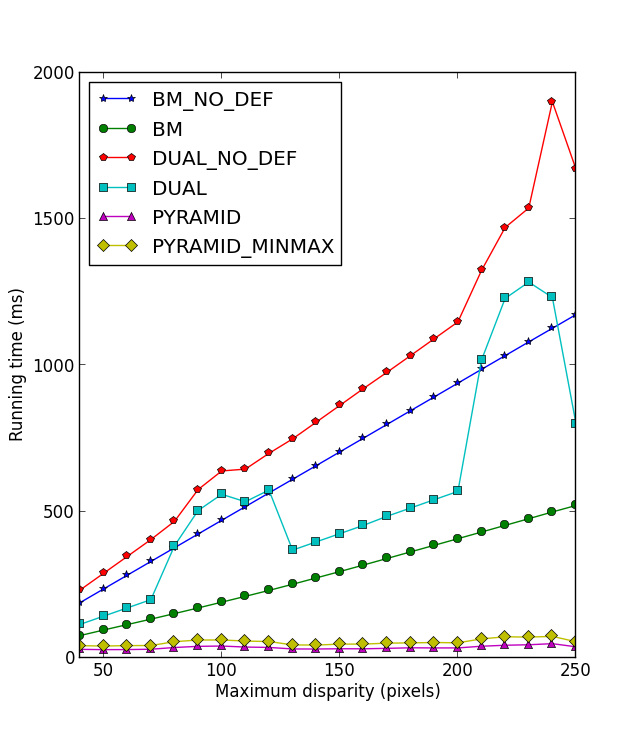
\includegraphics[width=0.8\textwidth]{images/runtime_9.png}
  \caption{Running time for each algorithm}
  \label{runtime-9}
\end{figure}


\subsection{Disparity map quality}

\begin{figure}
  \centering
  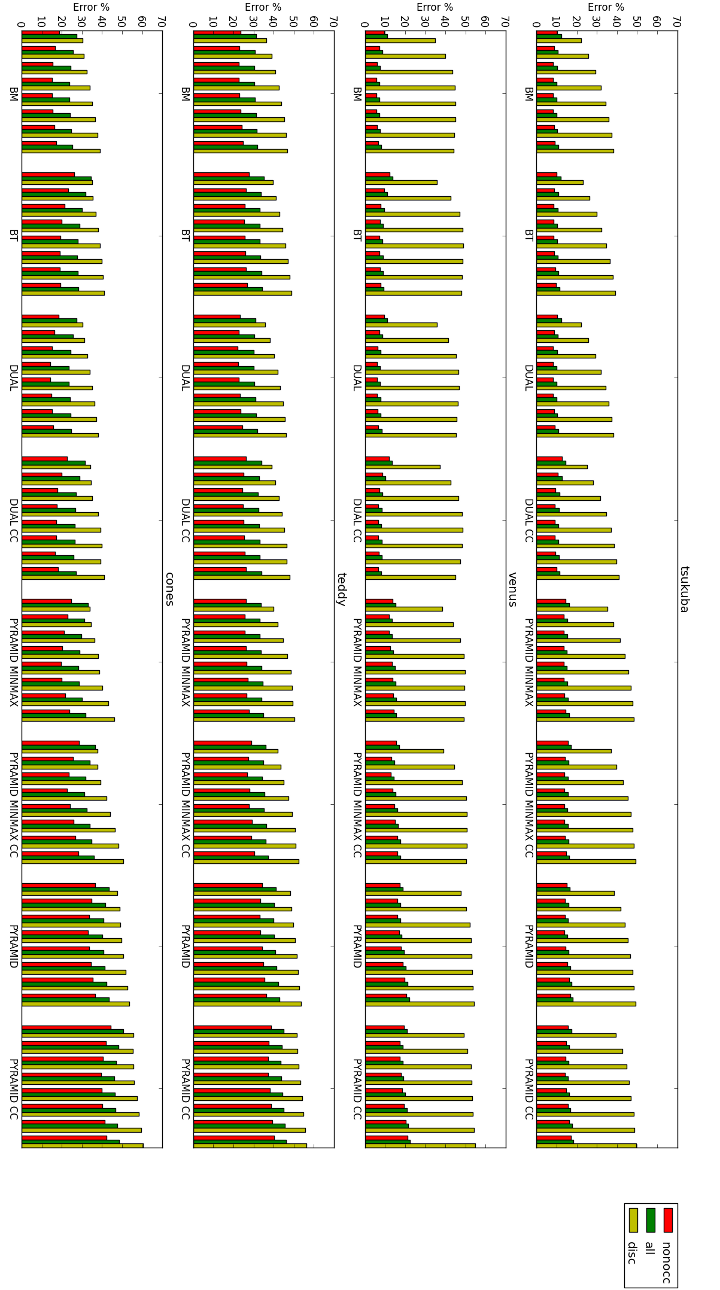
\includegraphics[width=\textwidth,height=\textheight]{images/quality_barchart_flipped.png}
  \caption{Error percentages for the datasets. Each graph contains
    groups of 3 * 8 bars, each representing increasing window sizes
    ranging from 7 up to 21 pixels}
  \label{quality-barchart}
\end{figure}


Figure \ref{quality-barchar} shows how the quality is affected by
increasing aggregation window size, $\omega$ $\times$ $\omega$. Each
of the four graphs are measurements on the four middlebury evaluation
datasets. In each graph, groups of 3 $\times$ 8 bars represent the
error percentages for non-occluded, all and discontinuity areas, with
increasing $\omega$ from 7 to 21. The algorithms used are labeled
beneath.

The notable features on the graph is the opposite trends of errors in
textureless areas and occlusions. In all instances, the increase of
$\omega$ results in a close to linear increase in errors in
occluded areas, while non-occluded areas are relatively constant, with
a few exceptions where the error rates decrease slightly.

Another noteworthy feature is that the algorithms using cross-checking
[TODO: ref cross-checking section] receives a higher error percentage
for occluded areas than the same algorithms without cross-checking.
This is because the evaluator also counts a disparity value of 0 as an
error, even in occluded areas. Non of the implemented algorithms
attempt to extrapolate disparities for occlusions, and therefor suffer
a higher error rate.

The algorithms not using cross-checking ends up with some disparity
value anywhere between 0 and max-disparity, which can be within the
threshold of what the evaluator considers an error. This can make the
cross-checking algorithms appear worse than its non-cross-checking
counterpart.

\begin{figure}
  \centering
  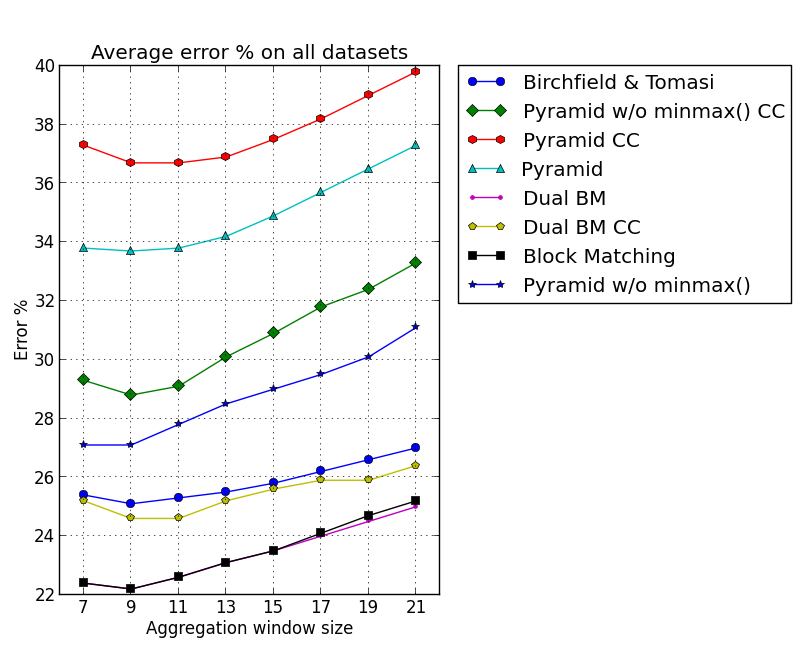
\includegraphics[width=\textwidth]{images/avg_error_all.png}
  \caption{Average error percentages for all the datasets. }
  \label{average-error-rates-final}
\end{figure}

The overall best quality is found by averaging error rates over all
four datasets, as shown in figure\ref{average-error-rates-final}. As
with most local algorithms, averaging the error rates is a trade-off
between the type of errors one considers most important.



\begin{figure}

  \setcounter{subfigure}{0}
  \label{fig:grid-of-outputs-tsukuba}
  \centering


  \begin{subfigure}[b]{0.45\textwidth}
    \centering
    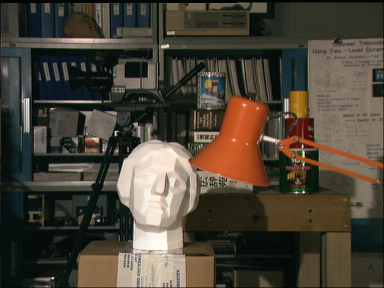
\includegraphics[width=\textwidth]{images/stereo-pairs/tsukuba_imL.png}
    \caption{Input}
  \end{subfigure}
  ~
  \begin{subfigure}[b]{0.45\textwidth}
    \centering
    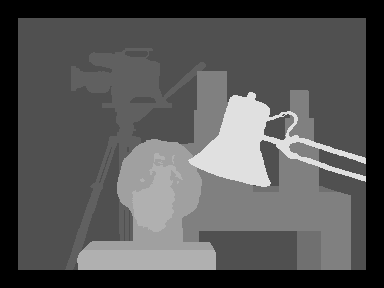
\includegraphics[width=\textwidth]{images/stereo-pairs/tsukuba_groundtruth.png}
    \caption{Ground truth}
  \end{subfigure}

  %
  %

  \begin{subfigure}[b]{0.23\textwidth}
    \centering
    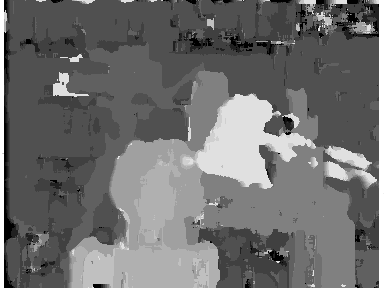
\includegraphics[width=\textwidth]{images/stereo-pairs/tsukuba_bm_9.png}
    \caption{BM 9}
  \end{subfigure}
  ~
  \begin{subfigure}[b]{0.23\textwidth}
    \centering
    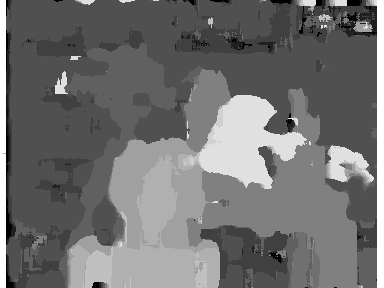
\includegraphics[width=\textwidth]{images/stereo-pairs/tsukuba_bm_13.png}
    \caption{BM 13}
  \end{subfigure}
  ~
  \begin{subfigure}[b]{0.23\textwidth}
    \centering
    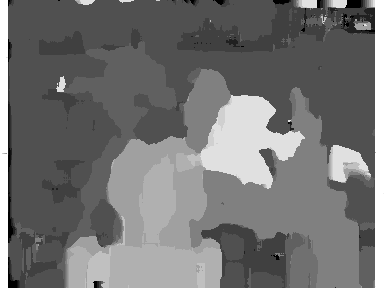
\includegraphics[width=\textwidth]{images/stereo-pairs/tsukuba_bm_17.png}
    \caption{BM 17}
  \end{subfigure}
  ~
  \begin{subfigure}[b]{0.23\textwidth}
    \centering
    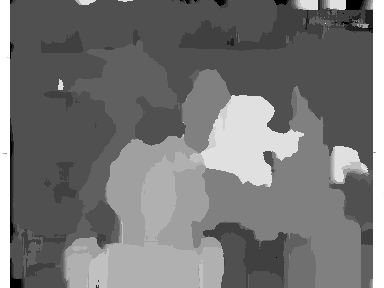
\includegraphics[width=\textwidth]{images/stereo-pairs/tsukuba_bm_21.png}
    \caption{BM 21}
  \end{subfigure}

  %
  %

  \begin{subfigure}[b]{0.23\textwidth}
    \centering
    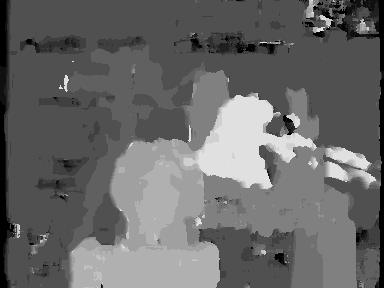
\includegraphics[width=\textwidth]{images/stereo-pairs/tsukuba_bt_9.png}
    \caption{BT 9}
  \end{subfigure}
  ~
  \begin{subfigure}[b]{0.23\textwidth}
    \centering
    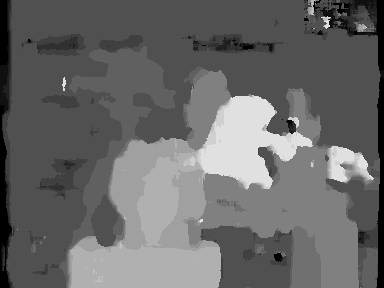
\includegraphics[width=\textwidth]{images/stereo-pairs/tsukuba_bt_13.png}
    \caption{BT 13}
  \end{subfigure}
  ~
  \begin{subfigure}[b]{0.23\textwidth}
    \centering
    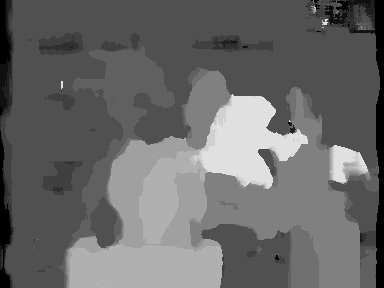
\includegraphics[width=\textwidth]{images/stereo-pairs/tsukuba_bt_17.png}
    \caption{BT 17}
  \end{subfigure}
  ~
  \begin{subfigure}[b]{0.23\textwidth}
    \centering
    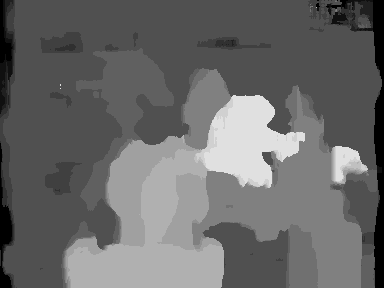
\includegraphics[width=\textwidth]{images/stereo-pairs/tsukuba_bt_21.png}
    \caption{BT 21}
  \end{subfigure}

  %
  %

  \begin{subfigure}[b]{0.23\textwidth}
    \centering
    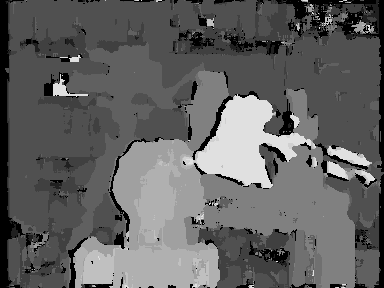
\includegraphics[width=\textwidth]{images/stereo-pairs/tsukuba_dual_crosschecked_9.png}
    \caption{CC 9}
  \end{subfigure}
  ~
  \begin{subfigure}[b]{0.23\textwidth}
    \centering
    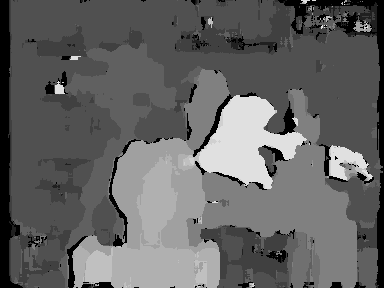
\includegraphics[width=\textwidth]{images/stereo-pairs/tsukuba_dual_crosschecked_13.png}
    \caption{CC 13}
  \end{subfigure}
  ~
  \begin{subfigure}[b]{0.23\textwidth}
    \centering
    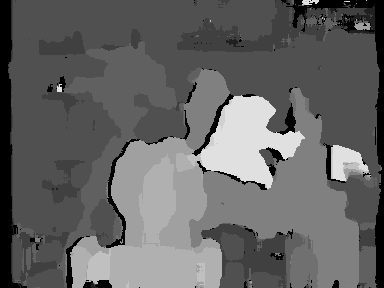
\includegraphics[width=\textwidth]{images/stereo-pairs/tsukuba_dual_crosschecked_17.png}
    \caption{CC 17}
  \end{subfigure}
  ~
  \begin{subfigure}[b]{0.23\textwidth}
    \centering
    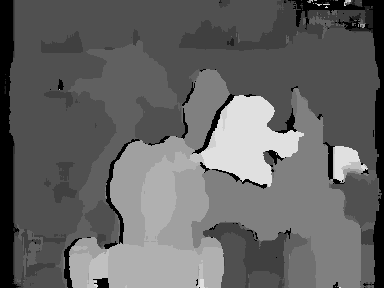
\includegraphics[width=\textwidth]{images/stereo-pairs/tsukuba_dual_crosschecked_21.png}
    \caption{CC 21}
  \end{subfigure}

  %
  %

  \begin{subfigure}[b]{0.23\textwidth}
    \centering
    
\includegraphics[width=\textwidth]{images/stereo-pairs/tsukuba_pyramid_9.png}
    \caption{PY 9}
  \end{subfigure}
  ~
  \begin{subfigure}[b]{0.23\textwidth}
    \centering
    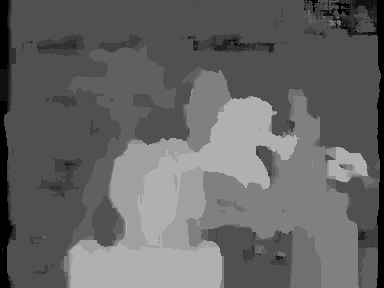
\includegraphics[width=\textwidth]{images/stereo-pairs/tsukuba_pyramid_13.png}
    \caption{PY 13}
  \end{subfigure}
  ~
  \begin{subfigure}[b]{0.23\textwidth}
    \centering
    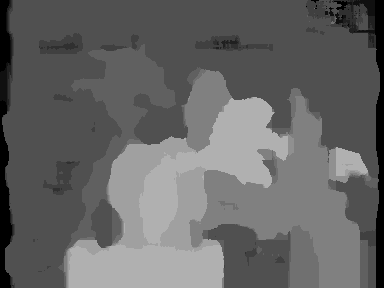
\includegraphics[width=\textwidth]{images/stereo-pairs/tsukuba_pyramid_17.png}
    \caption{PY 17}
  \end{subfigure}
  ~
  \begin{subfigure}[b]{0.23\textwidth}
    \centering
    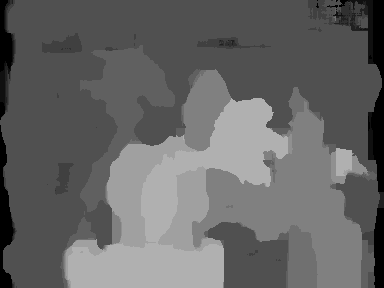
\includegraphics[width=\textwidth]{images/stereo-pairs/tsukuba_pyramid_21.png}
    \caption{PY 21}
  \end{subfigure}

  %
  %

  \begin{subfigure}[b]{0.23\textwidth}
    \centering
    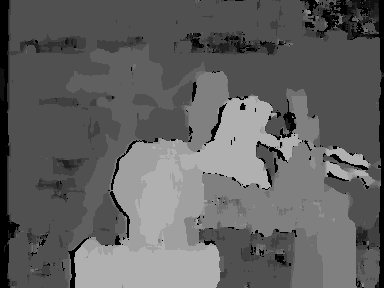
\includegraphics[width=\textwidth]{images/stereo-pairs/tsukuba_pyramid_crosschecked_9.png}
    \caption{PY CC 9}
  \end{subfigure}
  ~
  \begin{subfigure}[b]{0.23\textwidth}
    \centering
    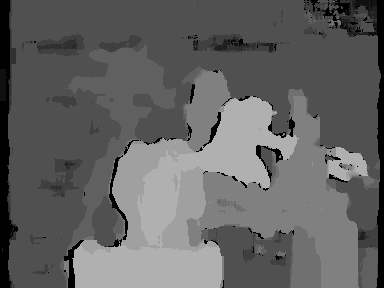
\includegraphics[width=\textwidth]{images/stereo-pairs/tsukuba_pyramid_crosschecked_13.png}
    \caption{PY CC 13}
  \end{subfigure}
  ~
  \begin{subfigure}[b]{0.23\textwidth}
    \centering
    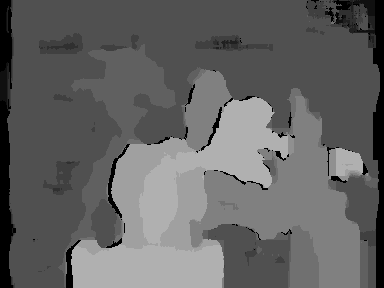
\includegraphics[width=\textwidth]{images/stereo-pairs/tsukuba_pyramid_crosschecked_17.png}
    \caption{PY CC 17}
  \end{subfigure}
  ~
  \begin{subfigure}[b]{0.23\textwidth}
    \centering
    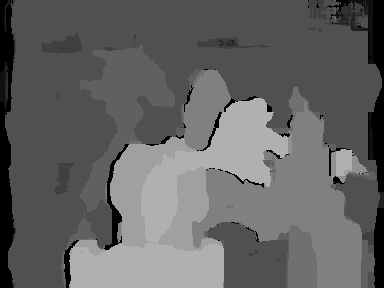
\includegraphics[width=\textwidth]{images/stereo-pairs/tsukuba_pyramid_crosschecked_21.png}
    \caption{PY CC 21}
  \end{subfigure}

  \caption{Tsukuba dataset}

\end{figure}



\begin{figure}
  \setcounter{subfigure}{0}
  \label{fig:grid-of-outputs-venus}
  \centering



  \begin{subfigure}[b]{0.3\textwidth}
    \centering
    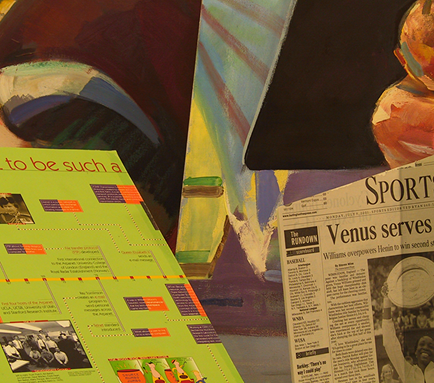
\includegraphics[width=\textwidth]{images/stereo-pairs/venus_imL.png}
    \caption{Input}
  \end{subfigure}
  ~
  \begin{subfigure}[b]{0.3\textwidth}
    \centering
    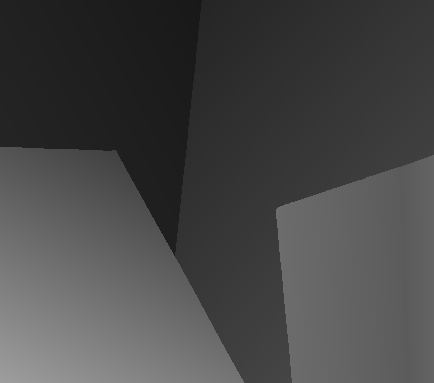
\includegraphics[width=\textwidth]{images/stereo-pairs/venus_groundtruth.png}
    \caption{Ground truth}
  \end{subfigure}

  %
  %

  \begin{subfigure}[b]{0.23\textwidth}
    \centering
    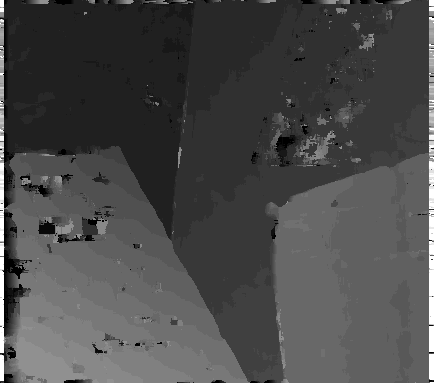
\includegraphics[width=\textwidth]{images/stereo-pairs/venus_bm_9.png}
    \caption{BM 9}
  \end{subfigure}
  ~
  \begin{subfigure}[b]{0.23\textwidth}
    \centering
    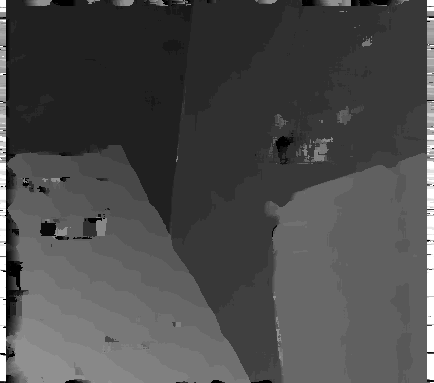
\includegraphics[width=\textwidth]{images/stereo-pairs/venus_bm_13.png}
    \caption{BM 13}
  \end{subfigure}
  ~
  \begin{subfigure}[b]{0.23\textwidth}
    \centering
    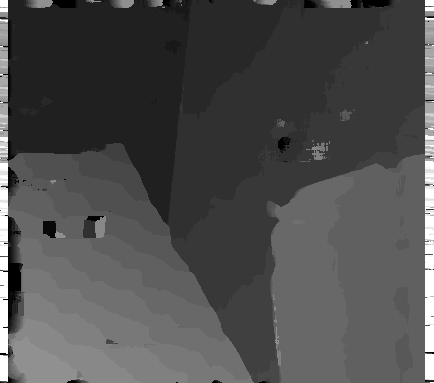
\includegraphics[width=\textwidth]{images/stereo-pairs/venus_bm_17.png}
    \caption{BM 17}
  \end{subfigure}
  ~
  \begin{subfigure}[b]{0.23\textwidth}
    \centering
    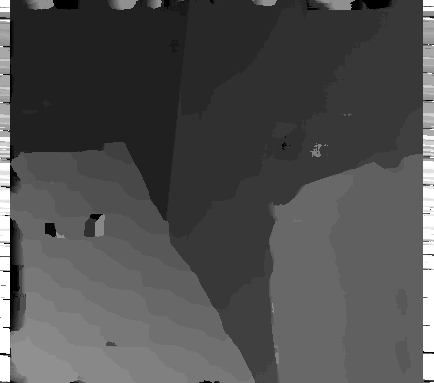
\includegraphics[width=\textwidth]{images/stereo-pairs/venus_bm_21.png}
    \caption{BM 21}
  \end{subfigure}

  %
  %

  \begin{subfigure}[b]{0.23\textwidth}
    \centering
    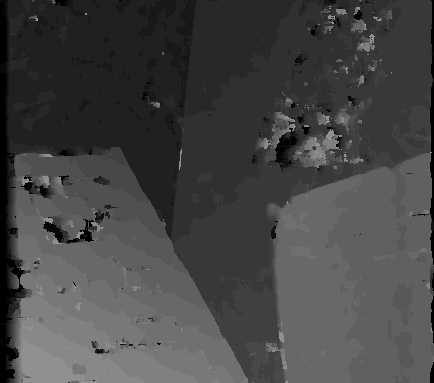
\includegraphics[width=\textwidth]{images/stereo-pairs/venus_bt_9.png}
    \caption{BT 9}
  \end{subfigure}
  ~
  \begin{subfigure}[b]{0.23\textwidth}
    \centering
    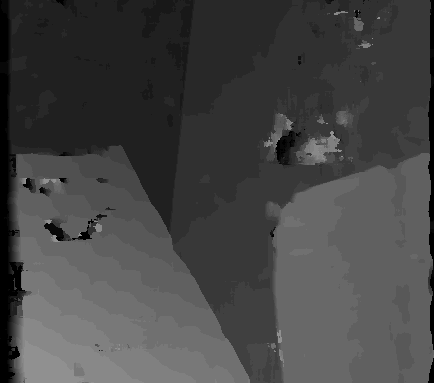
\includegraphics[width=\textwidth]{images/stereo-pairs/venus_bt_13.png}
    \caption{BT 13}
  \end{subfigure}
  ~
  \begin{subfigure}[b]{0.23\textwidth}
    \centering
    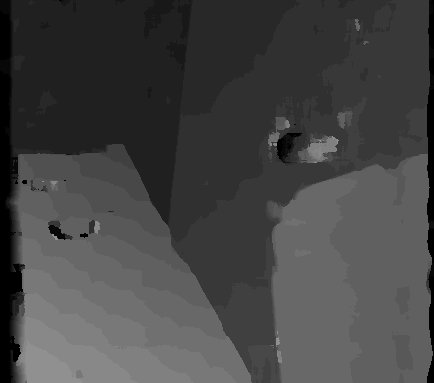
\includegraphics[width=\textwidth]{images/stereo-pairs/venus_bt_17.png}
    \caption{BT 17}
  \end{subfigure}
  ~
  \begin{subfigure}[b]{0.23\textwidth}
    \centering
    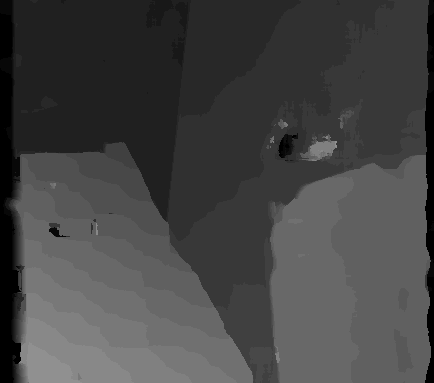
\includegraphics[width=\textwidth]{images/stereo-pairs/venus_bt_21.png}
    \caption{BT 21}
  \end{subfigure}

  %
  %

  \begin{subfigure}[b]{0.23\textwidth}
    \centering
    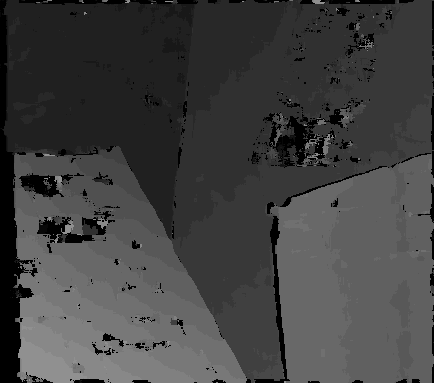
\includegraphics[width=\textwidth]{images/stereo-pairs/venus_dual_crosschecked_9.png}
    \caption{CC 9}
  \end{subfigure}
  ~
  \begin{subfigure}[b]{0.23\textwidth}
    \centering
    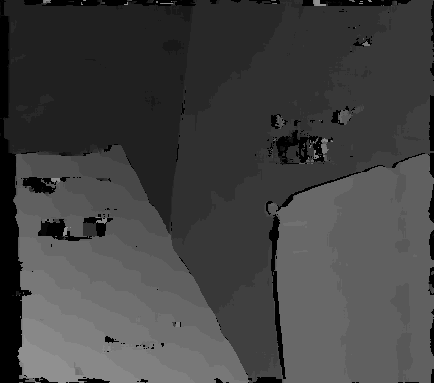
\includegraphics[width=\textwidth]{images/stereo-pairs/venus_dual_crosschecked_13.png}
    \caption{CC 13}
  \end{subfigure}
  ~
  \begin{subfigure}[b]{0.23\textwidth}
    \centering
    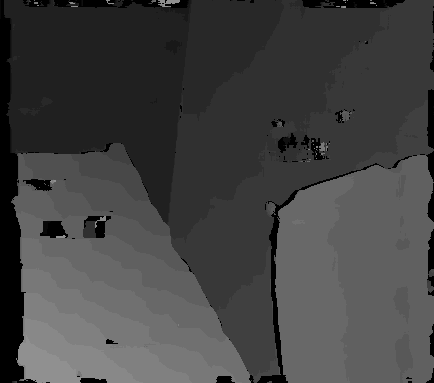
\includegraphics[width=\textwidth]{images/stereo-pairs/venus_dual_crosschecked_17.png}
    \caption{CC 17}
  \end{subfigure}
  ~
  \begin{subfigure}[b]{0.23\textwidth}
    \centering
    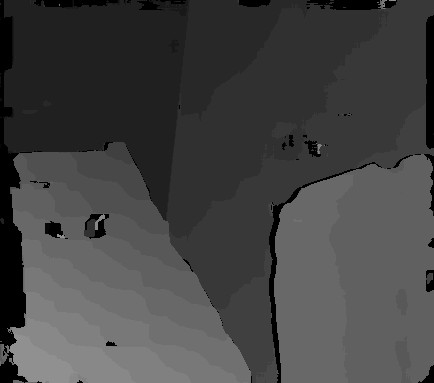
\includegraphics[width=\textwidth]{images/stereo-pairs/venus_dual_crosschecked_21.png}
    \caption{CC 21}
  \end{subfigure}

  %
  %

  \begin{subfigure}[b]{0.23\textwidth}
    \centering
    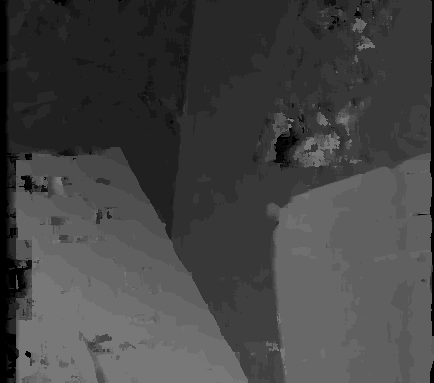
\includegraphics[width=\textwidth]{images/stereo-pairs/venus_pyramid_9.png}
    \caption{PY 9}
  \end{subfigure}
  ~
  \begin{subfigure}[b]{0.23\textwidth}
    \centering
    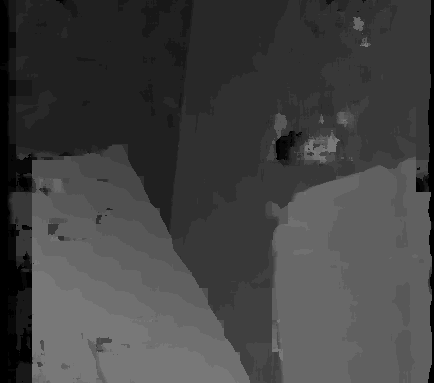
\includegraphics[width=\textwidth]{images/stereo-pairs/venus_pyramid_13.png}
    \caption{PY 13}
  \end{subfigure}
  ~
  \begin{subfigure}[b]{0.23\textwidth}
    \centering
    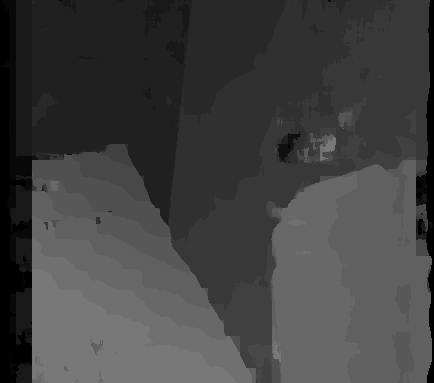
\includegraphics[width=\textwidth]{images/stereo-pairs/venus_pyramid_17.png}
    \caption{PY 17}
  \end{subfigure}
  ~
  \begin{subfigure}[b]{0.23\textwidth}
    \centering
    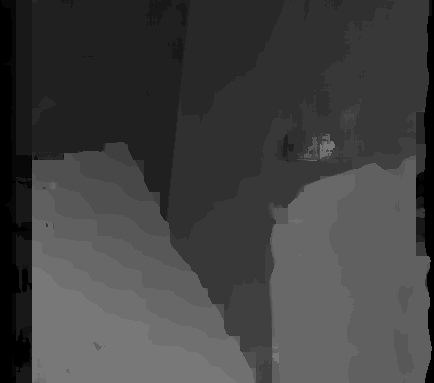
\includegraphics[width=\textwidth]{images/stereo-pairs/venus_pyramid_21.png}
    \caption{PY 21}
  \end{subfigure}

  %
  %

  \begin{subfigure}[b]{0.23\textwidth}
    \centering
    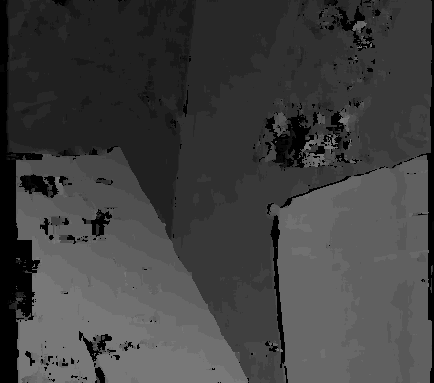
\includegraphics[width=\textwidth]{images/stereo-pairs/venus_pyramid_crosschecked_9.png}
    \caption{PY CC 9}
  \end{subfigure}
  ~
  \begin{subfigure}[b]{0.23\textwidth}
    \centering
    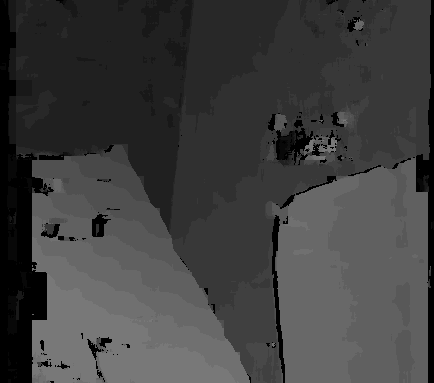
\includegraphics[width=\textwidth]{images/stereo-pairs/venus_pyramid_crosschecked_13.png}
    \caption{PY CC 13}
  \end{subfigure}
  ~
  \begin{subfigure}[b]{0.23\textwidth}
    \centering
    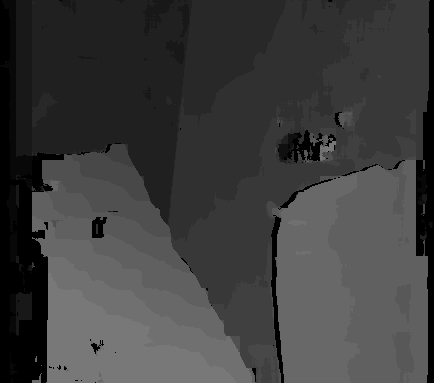
\includegraphics[width=\textwidth]{images/stereo-pairs/venus_pyramid_crosschecked_17.png}
    \caption{PY CC 17}
  \end{subfigure}
  ~
  \begin{subfigure}[b]{0.23\textwidth}
    \centering
    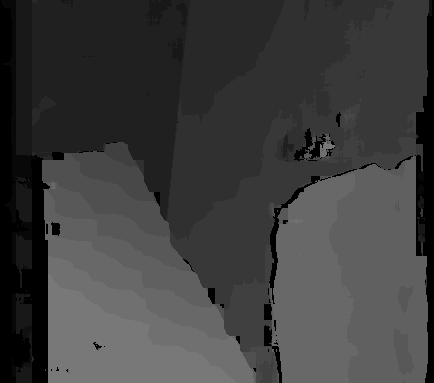
\includegraphics[width=\textwidth]{images/stereo-pairs/venus_pyramid_crosschecked_21.png}
    \caption{PY CC 21}
  \end{subfigure}

  \caption{Venus dataset}

\end{figure}

\begin{figure}
  \setcounter{subfigure}{0}

  \label{fig:grid-of-outputs-teddy}
  \centering


  \begin{subfigure}[b]{0.45\textwidth}
    \centering
    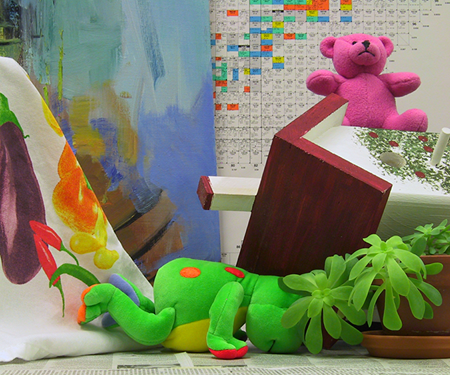
\includegraphics[width=\textwidth]{images/stereo-pairs/teddy_imL.png}
    \caption{Input}
  \end{subfigure}
  ~
  \begin{subfigure}[b]{0.45\textwidth}
    \centering
    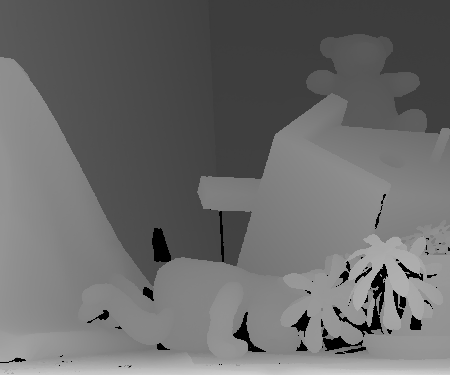
\includegraphics[width=\textwidth]{images/stereo-pairs/teddy_groundtruth.png}
    \caption{Ground truth}
  \end{subfigure}

  %
  %

  \begin{subfigure}[b]{0.23\textwidth}
    \centering
    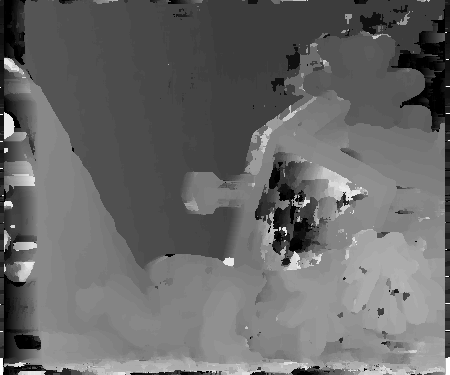
\includegraphics[width=\textwidth]{images/stereo-pairs/teddy_bm_9.png}
    \caption{BM 9}
  \end{subfigure}
  ~
  \begin{subfigure}[b]{0.23\textwidth}
    \centering
    \includegraphics[width=\textwidth]{images/stereo-pairs/teddy_bm_13.png}
    \caption{BM 13}
  \end{subfigure}
  ~
  \begin{subfigure}[b]{0.23\textwidth}
    \centering
    \includegraphics[width=\textwidth]{images/stereo-pairs/teddy_bm_17.png}
    \caption{BM 17}
  \end{subfigure}
  ~
  \begin{subfigure}[b]{0.23\textwidth}
    \centering
    \includegraphics[width=\textwidth]{images/stereo-pairs/teddy_bm_21.png}
    \caption{BM 21}
  \end{subfigure}




  \begin{subfigure}[b]{0.23\textwidth}
    \centering
    \includegraphics[width=\textwidth]{images/stereo-pairs/teddy_bt_9.png}
    \caption{BT 9}
  \end{subfigure}
  ~
  \begin{subfigure}[b]{0.23\textwidth}
    \centering
    \includegraphics[width=\textwidth]{images/stereo-pairs/teddy_bt_13.png}
    \caption{BT 13}
  \end{subfigure}
  ~
  \begin{subfigure}[b]{0.23\textwidth}
    \centering
    \includegraphics[width=\textwidth]{images/stereo-pairs/teddy_bt_17.png}
    \caption{BT 17}
  \end{subfigure}
  ~
  \begin{subfigure}[b]{0.23\textwidth}
    \centering
    \includegraphics[width=\textwidth]{images/stereo-pairs/teddy_bt_21.png}
    \caption{BT 21}
  \end{subfigure}




  \begin{subfigure}[b]{0.23\textwidth}
    \centering
    \includegraphics[width=\textwidth]{images/stereo-pairs/teddy_dual_crosschecked_9.png}
    \caption{CC 9}
  \end{subfigure}
  ~
  \begin{subfigure}[b]{0.23\textwidth}
    \centering
    \includegraphics[width=\textwidth]{images/stereo-pairs/teddy_dual_crosschecked_13.png}
    \caption{CC 13}
  \end{subfigure}
  ~
  \begin{subfigure}[b]{0.23\textwidth}
    \centering
    \includegraphics[width=\textwidth]{images/stereo-pairs/teddy_dual_crosschecked_17.png}
    \caption{CC 17}
  \end{subfigure}
  ~
  \begin{subfigure}[b]{0.23\textwidth}
    \centering
    \includegraphics[width=\textwidth]{images/stereo-pairs/teddy_dual_crosschecked_21.png}
    \caption{CC 21}
  \end{subfigure}




  \begin{subfigure}[b]{0.23\textwidth}
    \centering
    \includegraphics[width=\textwidth]{images/stereo-pairs/teddy_pyramid_9.png}
    \caption{PY 9}
  \end{subfigure}
  ~
  \begin{subfigure}[b]{0.23\textwidth}
    \centering
    \includegraphics[width=\textwidth]{images/stereo-pairs/teddy_pyramid_13.png}
    \caption{PY 13}
  \end{subfigure}
  ~
  \begin{subfigure}[b]{0.23\textwidth}
    \centering
    \includegraphics[width=\textwidth]{images/stereo-pairs/teddy_pyramid_17.png}
    \caption{PY 17}
  \end{subfigure}
  ~
  \begin{subfigure}[b]{0.23\textwidth}
    \centering
    \includegraphics[width=\textwidth]{images/stereo-pairs/teddy_pyramid_21.png}
    \caption{PY 21}
  \end{subfigure}




  \begin{subfigure}[b]{0.23\textwidth}
    \centering
    \includegraphics[width=\textwidth]{images/stereo-pairs/teddy_pyramid_crosschecked_9.png}
    \caption{PY CC 9}
  \end{subfigure}
  ~
  \begin{subfigure}[b]{0.23\textwidth}
    \centering
    \includegraphics[width=\textwidth]{images/stereo-pairs/teddy_pyramid_crosschecked_13.png}
    \caption{PY CC 13}
  \end{subfigure}
  ~
  \begin{subfigure}[b]{0.23\textwidth}
    \centering
    \includegraphics[width=\textwidth]{images/stereo-pairs/teddy_pyramid_crosschecked_17.png}
    \caption{PY CC 17}
  \end{subfigure}
  ~
  \begin{subfigure}[b]{0.23\textwidth}
    \centering
    \includegraphics[width=\textwidth]{images/stereo-pairs/teddy_pyramid_crosschecked_21.png}
    \caption{PY CC 21}
  \end{subfigure}

  \caption{Teddy dataset}

\end{figure}


\begin{figure}
  \setcounter{subfigure}{0}

  \label{fig:grid-of-outputs-cones}
  \centering


  \begin{subfigure}[b]{0.45\textwidth}
    \centering
    \includegraphics[width=\textwidth]{images/stereo-pairs/cones_imL.png}
    \caption{Input}
  \end{subfigure}
  ~
  \begin{subfigure}[b]{0.45\textwidth}
    \centering
    \includegraphics[width=\textwidth]{images/stereo-pairs/cones_groundtruth.png}
    \caption{Ground truth}
  \end{subfigure}

  %
  %

  \begin{subfigure}[b]{0.23\textwidth}
    \centering
    \includegraphics[width=\textwidth]{images/stereo-pairs/cones_bm_9.png}
    \caption{BM 9}
  \end{subfigure}
  ~
  \begin{subfigure}[b]{0.23\textwidth}
    \centering
    \includegraphics[width=\textwidth]{images/stereo-pairs/cones_bm_13.png}
    \caption{BM 13}
  \end{subfigure}
  ~
  \begin{subfigure}[b]{0.23\textwidth}
    \centering
    \includegraphics[width=\textwidth]{images/stereo-pairs/cones_bm_17.png}
    \caption{BM 17}
  \end{subfigure}
  ~
  \begin{subfigure}[b]{0.23\textwidth}
    \centering
    \includegraphics[width=\textwidth]{images/stereo-pairs/cones_bm_21.png}
    \caption{BM 21}
  \end{subfigure}

  %
  %

  \begin{subfigure}[b]{0.23\textwidth}
    \centering
    \includegraphics[width=\textwidth]{images/stereo-pairs/cones_bt_9.png}
    \caption{BT 9}
  \end{subfigure}
  ~
  \begin{subfigure}[b]{0.23\textwidth}
    \centering
    \includegraphics[width=\textwidth]{images/stereo-pairs/cones_bt_13.png}
    \caption{BT 13}
  \end{subfigure}
  ~
  \begin{subfigure}[b]{0.23\textwidth}
    \centering
    \includegraphics[width=\textwidth]{images/stereo-pairs/cones_bt_17.png}
    \caption{BT 17}
  \end{subfigure}
  ~
  \begin{subfigure}[b]{0.23\textwidth}
    \centering
    \includegraphics[width=\textwidth]{images/stereo-pairs/cones_bt_21.png}
    \caption{BT 21}
  \end{subfigure}

  %
  %

  \begin{subfigure}[b]{0.23\textwidth}
    \centering
    \includegraphics[width=\textwidth]{images/stereo-pairs/cones_dual_crosschecked_9.png}
    \caption{CC 9}
  \end{subfigure}
  ~
  \begin{subfigure}[b]{0.23\textwidth}
    \centering
    \includegraphics[width=\textwidth]{images/stereo-pairs/cones_dual_crosschecked_13.png}
    \caption{CC 13}
  \end{subfigure}
  ~
  \begin{subfigure}[b]{0.23\textwidth}
    \centering
    \includegraphics[width=\textwidth]{images/stereo-pairs/cones_dual_crosschecked_17.png}
    \caption{CC 17}
  \end{subfigure}
  ~
  \begin{subfigure}[b]{0.23\textwidth}
    \centering
    \includegraphics[width=\textwidth]{images/stereo-pairs/cones_dual_crosschecked_21.png}
    \caption{CC 21}
  \end{subfigure}

  %
  %

  \begin{subfigure}[b]{0.23\textwidth}
    \centering
    \includegraphics[width=\textwidth]{images/stereo-pairs/cones_pyramid_9.png}
    \caption{PY 9}
  \end{subfigure}
  ~
  \begin{subfigure}[b]{0.23\textwidth}
    \centering
    \includegraphics[width=\textwidth]{images/stereo-pairs/cones_pyramid_13.png}
    \caption{PY 13}
  \end{subfigure}
  ~
  \begin{subfigure}[b]{0.23\textwidth}
    \centering
    \includegraphics[width=\textwidth]{images/stereo-pairs/cones_pyramid_17.png}
    \caption{PY 17}
  \end{subfigure}
  ~
  \begin{subfigure}[b]{0.23\textwidth}
    \centering
    \includegraphics[width=\textwidth]{images/stereo-pairs/cones_pyramid_21.png}
    \caption{PY 21}
  \end{subfigure}

  %
  %

  \begin{subfigure}[b]{0.23\textwidth}
    \centering
    \includegraphics[width=\textwidth]{images/stereo-pairs/cones_pyramid_crosschecked_9.png}
    \caption{PY CC 9}
  \end{subfigure}
  ~
  \begin{subfigure}[b]{0.23\textwidth}
    \centering
    \includegraphics[width=\textwidth]{images/stereo-pairs/cones_pyramid_crosschecked_13.png}
    \caption{PY CC 13}
  \end{subfigure}
  ~
  \begin{subfigure}[b]{0.23\textwidth}
    \centering
    \includegraphics[width=\textwidth]{images/stereo-pairs/cones_pyramid_crosschecked_17.png}
    \caption{PY CC 17}
  \end{subfigure}
  ~
  \begin{subfigure}[b]{0.23\textwidth}
    \centering
    \includegraphics[width=\textwidth]{images/stereo-pairs/cones_pyramid_crosschecked_21.png}
    \caption{PY CC 21}
  \end{subfigure}

  \caption{Cones dataset}

\end{figure}

\begin{table}
    \begin{tabular}{|l|l|l|l|l|l|l|}
        \hline
        disparity & BM\_NO\_DEF & BM     & DUAL\_NO\_DEF & DUAL    & PYRAMID & MINMAX \\ \hline
        50 & 188.70    & 76.18  & 231.81      & 114.36  & 29.14   & 41.77          \\
        60 & 235.67    & 95.22  & 289.25      & 142.68  & 28.18   & 40.44          \\
        70 & 282.57    & 113.80 & 346.73      & 170.83  & 28.35   & 41.95          \\
        80 & 329.52    & 132.39 & 404.38      & 199.02  & 29.55   & 42.25          \\
        90 & 376.42    & 151.40 & 466.80      & 383.05  & 35.47   & 55.27          \\
        100 & 423.41    & 170.64 & 575.43      & 503.63  & 39.40   & 61.07          \\
       110 & 470.31    & 190.44 & 639.04      & 559.31  & 40.48   & 61.24          \\
        120 & 517.05    & 210.34 & 645.30      & 533.80  & 37.00   & 57.42          \\
        130 & 563.85    & 230.64 & 699.17      & 573.71  & 35.74   & 55.89          \\
        140 & 610.49    & 251.62 & 748.59      & 368.40  & 30.46   & 44.37          \\
        150 & 657.21    & 273.35 & 805.79      & 396.54  & 30.31   & 43.71          \\
        160 & 704.13    & 295.04 & 863.08      & 424.75  & 31.18   & 47.09          \\
        170 & 751.17    & 317.43 & 920.68      & 453.04  & 31.02   & 47.12          \\
        180 & 798.22    & 339.84 & 976.49      & 484.16  & 32.58   & 50.35          \\
        190 & 845.26    & 362.44 & 1033.66     & 512.42  & 34.46   & 51.28          \\
        200 & 892.14    & 384.89 & 1091.29     & 540.90  & 33.98   & 52.54          \\
        210 & 939.28    & 407.46 & 1148.60     & 569.16  & 34.04   & 51.51          \\
        220 & 986.41    & 430.19 & 1324.52     & 1018.30 & 39.81   & 64.96          \\
        230 & 1033.23   & 453.00 & 1471.33     & 1229.00 & 43.17   & 72.08          \\
        240 & 1080.22   & 475.77 & 1538.02     & 1284.77 & 44.88   & 71.05          \\
        250 & 1126.74   & 498.85 & 1901.21     & 1232.11 & 48.57   & 73.48          \\
        \hline
    \end{tabular}
    \caption{Run times in milliseconds for each algorithm run at
      increasing search ranges}
\end{table}

\begin{tabular}{|l|l|l||l|l|l||l|l|l||l|l|l||l|}
  \hline
  \multicolumn{3}{|c||}{Tsukuba} &
  \multicolumn{3}{c||}{Venus} &
  \multicolumn{3}{c||}{Teddy} &
  \multicolumn{3}{c||}{Cones} & ~ \\
  \hline
  nocc & all & disc & nocc & all & disc & nocc & all & disc & nocc & all & disc & avg err\\
  \hline
  \multicolumn{13}{|c|}{Normal Block Matching} \\
  \hline
  10.4 & 12.3 & 22.3 & 9.62 & 11.1 & 35.0 & 23.6 & 31.3 & 36.4 & 18.8 & 27.5 & 30.2 & 22.4 \\
  8.79 & 10.7 & 25.7 & 7.14 & 8.67 & 40.1 & 22.9 & 30.6 & 38.9 & 16.7 & 25.6 & 30.9 & 22.2 \\
  8.24 & 10.2 & 29.4 & 6.17 & 7.69 & 43.6 & 22.6 & 30.3 & 40.7 & 15.6 & 24.4 & 32.4 & 22.6 \\
  8.09 & 9.91 & 32.1 & 5.79 & 7.30 & 44.9 & 22.8 & 30.5 & 42.6 & 15.1 & 23.9 & 33.9 & 23.1 \\
  8.14 & 9.88 & 34.3 & 5.70 & 7.19 & 45.2 & 23.1 & 30.8 & 43.9 & 15.1 & 23.8 & 35.1 & 23.5 \\
  8.33 & 10.0 & 36.0 & 5.84 & 7.30 & 45.0 & 23.6 & 31.2 & 45.3 & 15.6 & 24.2 & 36.5 & 24.1 \\
  8.76 & 10.4 & 37.4 & 6.10 & 7.54 & 44.6 & 24.1 & 31.6 & 46.2 & 16.4 & 24.8 & 37.9 & 24.7 \\
  9.24 & 10.9 & 38.4 & 6.61 & 8.02 & 44.1 & 24.7 & 32.0 & 46.8 & 17.1 & 25.3 & 38.9 & 25.2 \\
  \hline
  \multicolumn{13}{|c|}{Block Matching with Birchfield \& Tomasi matching} \\
  \hline
  10.1 & 12.0 & 23.0 & 12.4 & 13.9 & 35.8 & 27.6 & 35.1 & 39.7 & 26.2 & 34.4 & 35.0 & 25.4 \\
  8.92 & 10.9 & 26.4 & 9.54 & 11.1 & 42.8 & 26.2 & 33.7 & 41.2 & 23.2 & 31.7 & 35.4 & 25.1 \\
  8.58 & 10.6 & 29.8 & 7.95 & 9.52 & 47.2 & 25.6 & 33.2 & 43.0 & 21.5 & 30.1 & 36.8 & 25.3 \\
  8.51 & 10.4 & 32.4 & 7.43 & 9.00 & 48.6 & 25.4 & 33.0 & 44.4 & 20.0 & 28.8 & 38.0 & 25.5 \\
  8.61 & 10.4 & 34.6 & 7.28 & 8.84 & 48.9 & 25.5 & 33.1 & 45.8 & 19.2 & 28.0 & 39.0 & 25.8 \\
  8.83 & 10.6 & 36.4 & 7.34 & 8.91 & 48.7 & 25.9 & 33.5 & 47.2 & 19.0 & 27.8 & 39.9 & 26.2 \\
  9.26 & 11.0 & 38.0 & 7.50 & 9.09 & 48.3 & 26.3 & 33.9 & 48.1 & 19.1 & 27.9 & 40.5 & 26.6 \\
  9.67 & 11.4 & 39.2 & 7.74 & 9.33 & 48.0 & 26.9 & 34.4 & 48.8 & 19.4 & 28.2 & 41.2 & 27.0 \\
  \hline
  \multicolumn{13}{|c|}{Block Matching with left \& right disparity map} \\
  \hline
  10.4 & 12.3 & 22.3 & 9.71 & 11.2 & 35.9 & 23.4 & 31.1 & 35.9 & 18.5 & 27.4 & 30.2 & 22.4 \\
  8.79 & 10.7 & 25.7 & 7.27 & 8.85 & 41.5 & 22.7 & 30.4 & 38.1 & 16.3 & 25.5 & 31.1 & 22.2 \\
  8.24 & 10.2 & 29.4 & 6.34 & 7.93 & 45.3 & 22.2 & 30.0 & 40.1 & 15.1 & 24.3 & 32.6 & 22.6 \\
  8.09 & 9.91 & 32.1 & 6.00 & 7.60 & 46.7 & 22.4 & 30.1 & 41.9 & 14.4 & 23.6 & 34.0 & 23.1 \\
  8.14 & 9.88 & 34.3 & 5.94 & 7.54 & 46.8 & 22.8 & 30.4 & 43.2 & 14.2 & 23.4 & 35.1 & 23.5 \\
  8.33 & 10.0 & 36.0 & 6.11 & 7.70 & 46.3 & 23.3 & 30.9 & 44.7 & 14.8 & 24.0 & 36.2 & 24.0 \\
  8.76 & 10.4 & 37.4 & 6.39 & 7.98 & 45.8 & 23.6 & 31.3 & 45.6 & 15.3 & 24.4 & 37.3 & 24.5 \\
  9.24 & 10.9 & 38.4 & 6.71 & 8.30 & 45.3 & 24.4 & 31.9 & 46.2 & 15.8 & 24.8 & 38.0 & 25.0 \\
  \hline
  \multicolumn{13}{|c|}{Block Matching with left \& right disparity map and cross-checking} \\
  \hline
  12.6 & 14.6 & 25.3 & 12.0 & 13.5 & 37.3 & 26.2 & 33.9 & 39.1 & 22.7 & 31.5 & 34.1 & 25.2 \\
  10.5 & 12.6 & 28.3 & 8.69 & 10.3 & 42.8 & 25.1 & 32.8 & 40.8 & 19.9 & 29.0 & 34.6 & 24.6 \\
  9.47 & 11.5 & 31.7 & 7.27 & 8.88 & 46.6 & 24.4 & 32.2 & 42.7 & 17.9 & 27.2 & 35.0 & 24.6 \\
  9.13 & 11.1 & 34.6 & 6.77 & 8.40 & 48.3 & 24.7 & 32.5 & 44.1 & 17.4 & 26.7 & 38.2 & 25.2 \\
  9.04 & 10.9 & 37.0 & 6.66 & 8.28 & 48.7 & 25.1 & 32.8 & 45.4 & 17.2 & 26.5 & 39.4 & 25.6 \\
  9.10 & 10.9 & 38.7 & 6.73 & 8.35 & 48.2 & 25.3 & 33.0 & 46.6 & 17.3 & 26.5 & 39.8 & 25.9 \\
  9.43 & 11.2 & 39.9 & 6.86 & 8.49 & 47.4 & 25.6 & 33.2 & 46.5 & 16.5 & 25.8 & 39.3 & 25.9 \\
  9.88 & 11.6 & 40.9 & 6.76 & 8.25 & 45.0 & 26.3 & 33.9 & 48.0 & 18.1 & 27.2 & 41.1 & 26.4 \\

  \hline
\end{tabular}

\begin{tabular}{|l|l|l||l|l|l||l|l|l||l|l|l||l|}
  \hline
  \multicolumn{3}{|c||}{Tsukuba} &
  \multicolumn{3}{c||}{Venus} &
  \multicolumn{3}{c||}{Teddy} &
  \multicolumn{3}{c||}{Cones} & ~ \\
  \hline
  nocc & all & disc & nocc & all & disc & nocc & all & disc & nocc & all & disc & avg err\\
  \hline
  \multicolumn{13}{|c|}{Pyramid with min-maxing} \\
  \hline
  14.6 & 16.2 & 35.3 & 13.8 & 15.3 & 38.5 & 26.3 & 33.8 & 39.9 & 24.8 & 33.1 & 33.8 & 27.1 \\
  13.7 & 15.4 & 38.3 & 11.9 & 13.4 & 43.8 & 25.5 & 33.1 & 42.0 & 22.8 & 31.2 & 34.5 & 27.1 \\
  13.5 & 15.2 & 41.6 & 12.0 & 13.4 & 47.5 & 25.5 & 33.2 & 44.7 & 21.1 & 29.7 & 36.3 & 27.8 \\
  13.5 & 15.0 & 43.9 & 12.6 & 14.1 & 49.2 & 26.1 & 33.6 & 46.9 & 20.2 & 28.9 & 38.0 & 28.5 \\
  13.5 & 15.1 & 45.6 & 13.6 & 15.1 & 49.7 & 26.5 & 34.0 & 48.5 & 19.7 & 28.4 & 38.8 & 29.0 \\
  13.7 & 15.2 & 46.9 & 13.7 & 15.2 & 49.4 & 27.1 & 34.5 & 49.2 & 20.0 & 28.6 & 40.2 & 29.5 \\
  14.0 & 15.5 & 47.7 & 14.2 & 15.6 & 49.9 & 26.6 & 34.1 & 49.4 & 21.7 & 30.0 & 43.2 & 30.1 \\
  14.6 & 16.1 & 48.5 & 14.3 & 15.7 & 49.2 & 27.6 & 35.0 & 50.3 & 23.8 & 31.9 & 46.0 & 31.1 \\
  \hline
  \multicolumn{13}{|c|}{Pyramid with min-maxing and cross-checking} \\
  \hline
  15.5 & 17.2 & 37.0 & 15.7 & 17.2 & 39.2 & 28.8 & 36.1 & 42.0 & 28.7 & 36.7 & 37.7 & 29.3 \\
  14.2 & 15.9 & 39.7 & 13.2 & 14.7 & 44.4 & 27.4 & 34.9 & 43.4 & 25.6 & 33.9 & 37.8 & 28.8 \\
  13.9 & 15.6 & 43.0 & 13.0 & 14.5 & 48.3 & 26.8 & 34.4 & 44.9 & 23.4 & 31.9 & 39.4 & 29.1 \\
  13.9 & 15.5 & 45.3 & 13.7 & 15.2 & 50.3 & 28.0 & 35.4 & 47.5 & 22.6 & 31.2 & 42.2 & 30.1 \\
  13.8 & 15.4 & 46.9 & 14.7 & 16.2 & 50.8 & 27.8 & 35.2 & 49.2 & 24.0 & 32.4 & 44.1 & 30.9 \\
  13.9 & 15.5 & 47.7 & 15.1 & 16.5 & 50.6 & 29.2 & 36.5 & 50.7 & 25.8 & 34.0 & 46.3 & 31.8 \\
  14.2 & 15.8 & 48.4 & 16.1 & 17.6 & 50.8 & 29.0 & 36.2 & 50.9 & 26.9 & 34.9 & 48.3 & 32.4 \\
  14.8 & 16.3 & 49.2 & 16.3 & 17.8 & 50.4 & 30.3 & 37.4 & 52.4 & 28.3 & 36.1 & 50.5 & 33.3 \\
  \hline
  \multicolumn{13}{|c|}{Pyramid} \\
  \hline
  15.0 & 16.6 & 38.7 & 17.4 & 18.8 & 47.8 & 34.3 & 41.0 & 48.2 & 36.5 & 43.4 & 47.7 & 33.8 \\
  14.2 & 15.8 & 41.8 & 16.2 & 17.6 & 50.3 & 33.5 & 40.3 & 49.0 & 34.8 & 41.8 & 48.7 & 33.7 \\
  14.1 & 15.6 & 43.9 & 16.3 & 17.7 & 52.2 & 33.2 & 40.0 & 49.7 & 33.6 & 40.7 & 49.2 & 33.8 \\
  13.9 & 15.4 & 45.3 & 17.0 & 18.4 & 52.7 & 33.5 & 40.3 & 50.8 & 33.1 & 40.3 & 49.8 & 34.2 \\
  14.6 & 16.0 & 46.6 & 18.0 & 19.4 & 53.0 & 34.2 & 40.9 & 51.6 & 33.6 & 40.7 & 50.5 & 34.9 \\
  15.4 & 16.7 & 47.9 & 18.8 & 20.2 & 53.4 & 34.9 & 41.5 & 52.2 & 34.6 & 41.5 & 51.7 & 35.7 \\
  16.2 & 17.4 & 48.5 & 19.7 & 21.1 & 53.8 & 35.6 & 42.2 & 52.7 & 35.5 & 42.3 & 52.7 & 36.5 \\
  16.9 & 18.0 & 49.3 & 20.7 & 22.0 & 54.3 & 36.3 & 42.8 & 53.5 & 36.7 & 43.3 & 53.7 & 37.3 \\
  \hline
  \multicolumn{13}{|c|}{Pyramid with cross-checking} \\
  \hline
  15.7 & 17.3 & 39.6 & 19.6 & 21.0 & 49.1 & 38.7 & 44.9 & 51.6 & 44.4 & 50.5 & 55.6 & 37.3 \\
  14.7 & 16.3 & 42.7 & 17.5 & 18.9 & 51.0 & 37.6 & 44.0 & 51.9 & 41.9 & 48.2 & 55.4 & 36.7 \\
  14.4 & 15.9 & 44.8 & 17.4 & 18.8 & 52.7 & 37.2 & 43.6 & 52.3 & 40.4 & 46.9 & 55.8 & 36.7 \\
  14.2 & 15.7 & 46.0 & 17.9 & 19.3 & 53.2 & 37.4 & 43.8 & 53.3 & 39.5 & 46.1 & 56.0 & 36.9 \\
  14.7 & 16.1 & 47.0 & 18.6 & 20.0 & 53.3 & 38.0 & 44.3 & 54.3 & 39.9 & 46.4 & 57.5 & 37.5 \\
  15.5 & 16.9 & 48.3 & 19.4 & 20.8 & 53.8 & 38.8 & 45.1 & 54.9 & 40.3 & 46.8 & 58.4 & 38.2 \\
  16.3 & 17.6 & 48.8 & 20.3 & 21.6 & 54.3 & 39.4 & 45.6 & 55.6 & 41.3 & 47.7 & 59.5 & 39.0 \\
  17.0 & 18.2 & 49.5 & 21.2 & 22.5 & 54.8 & 40.1 & 46.2 & 56.3 & 42.4 & 48.6 & 60.4 & 39.8 \\

  \hline
\end{tabular}


\section{Summary}

This chapter described the evolution of a block matching algorithm,
from a simple CPU proof-of-concept to a real time GPU implementation.



Future work: pyramid + GC, pyramid better pixel re-sampling,
refinement fill occlusions

Kristian Hagas Silhouette extraction thesis as a compute mask.
